\section{Barvení}
\subsection{Hranové obarvení}\label{hranObar}
Je dán graf bez smyček $G = (V,E, \eps)$ a konečná množina $C$ tzv. barev. \ii{Hranové obarvení} $G$ je přiřazení $c: E \rightarrow C$, že žádné dvě hrany se společným krajním vrcholem nemají stejnou barvu.

Lze také říci, že se snažíme graf pokrýt vzájemně disjunktními \hyperref[parovani]{párováními}.

\subsection{Hranová barevnost}\label{hranChrom}
Hranová barevnost, též \ii{chromatický index}, grafu $G$ je nejmenší počet barev, kterými lze \hyperref[hranObar]{hranově obarvit} graf $G$, značíme ji $\chi^\prime(G)$.

Nutně platí, že
\begin{equation}
    \chi^\prime(G) \geq \Delta(G).
\end{equation}

\subsection{Věta o souvislosti hranové barevnosti a maximálním stupni grafu}\label{vizing}
\ii{Vizing}. Je dán graf bez smyček $G = (V, E, \eps)$. Pak
\begin{equation}
    \Delta(G) \leq \chi^\prime (G) \leq \Delta(G) + 1.
\end{equation}
Bez důkazu.

\subsection{Vrcholové obarevní}\label{vrchObar}
Je dán prostý neorientovaný graf $G = (V,E)$ bez smyček a konečná množina $B$ (nazývaná též množina barev). \ii{Obarvení vrcholů} grafu (též \ii{vrcholové obarvení} grafu) je $b: V \rightarrow B$, že žádné dva vrcholy spojené hranou nemají stejnou barvu.

$G$ nazveme $k$-barevný, jestliže se dá obarvit $k$ barvami.

\subsection{Barevnost grafu}\label{vrchChrom}
Barevnost grafu $G$, též \ii{chromatické číslo} grafu $G$, je nejmenší $k$ takové, že $G$ je $k$-barevný, značíme ji $\chi(G)$.

\subsection{Tvrzení o dvoubarevném grafu}
Graf $G$ je dvoubarevný právě tehdy, když $G$ neobsahuje \hyperref[kruznice]{kružnici} liché délky, tedy $G$ je bipartitní.

\dukaz Ať $G = (V,E)$, $V = A \cup B$, tak, že:
\begin{align*}
    v \in A \iff \text{má barvu } 1 \\
    v \in B \iff \text{má barvu } 2 \\
\end{align*}
Stačí ukázat, že nemá-li $G$ kružnici liché délky, dá se obarvit 2 barvami.

Dokažme algoritmem barvení. Vyberme si počáteční vrchol $v$. Následně aplikujme algoritmus BFS (breath-first-search), kterým graf rozdělíme do několika úrovní. Každé úrovni přiřadíme barvu tak, že
\begin{equation}
    b(v) = 
    \begin{cases}
        1 \iff v \in H_{2i}, \\
        2 \iff v \in H_{2i+1}, \, \text{pro } i \in \N.   
    \end{cases}
\end{equation}

Kdyby $b$ nebylo obarvení; existuje $\bc{x, y} \in E$, kde $x \in H_i$ a $y \in H_j$ tak, že $i+j = 2k$, $k \in \N$.

V našem grafu existuje \hyperref[stc]{cesta} $P_i$ z $v$ do $x$ o $i$ hranách, a zároveň existuje cesta $P_j$ z $v$ do $y$ o $j$ hranách.

Když vezmeme $P_i$, $\bc{x,y}$, $P_j$ (pozpátku), jedná se o \hyperref[stc]{uzavřený sled} o $i+j+1=2k+1$ hranách.

Dále máme kružnici o $i+j+1-2\ell$ hranách, kde $\ell$ je počet hran ve \colorbox{green!30}{společném úseku $P_i, P_j$}.
\begin{figure}[H]
    \centering
    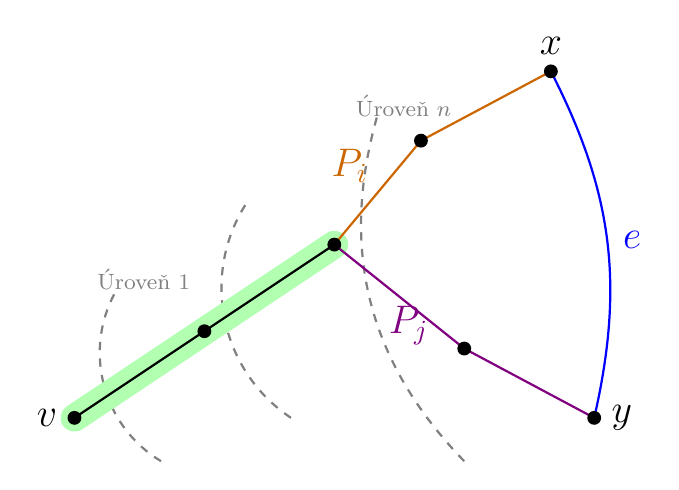
\begin{tikzpicture}[
        scale=1.1,
        vertex/.style={circle, fill=black, minimum size=5pt, inner sep=0pt},
        edge/.style={thick, line cap=round},
        highlight/.style={line width=10pt, green!30, line cap=round},
        level/.style={dashed, gray, thick}
    ]

        \coordinate (v) at (0, 0);
        \coordinate (n1) at (1.5, 1);
        \coordinate (split) at (3, 2);
        
        \coordinate (nx) at (4, 3.2);
        \coordinate (x) at (5.5, 4);
        \coordinate (ny) at (4.5, 0.8);
        \coordinate (y) at (6, 0);
        
        \draw[level] (1, -0.5) to[bend left=45] (0.5, 1.5);
        \node[gray, font=\footnotesize] at (0.8, 1.6) {Úroveň 1};
        
        \draw[level] (2.5, 0) to[bend left=45] (2, 2.5);
        
        \draw[level] (4.5, -0.5) to[bend left=30] (3.5, 3.5);
        \node[gray, font=\footnotesize] at (3.8, 3.6) {Úroveň $n$};

        \draw[highlight] (v) -- (n1) -- (split);

        \draw[edge] (v) -- (n1) -- (split);
        
        \draw[edge, orange!80!black] (split) -- (nx) -- (x);
        \node[above left, orange!80!black] at (3.5, 2.6) {\Large $P_i$};
        
        \draw[edge, violet] (split) -- (ny) -- (y);
        \node[below left, violet] at (4.2, 1.4) {\Large $P_j$};

        \draw[edge, blue] (x) to[bend left=20] node[midway, right, xshift=2pt] {\Large $e$} (y);

        \node[vertex, label=left:\Large $v$] at (v) {};
        \node[vertex] at (n1) {};
        \node[vertex] at (split) {};
        \node[vertex] at (nx) {};
        \node[vertex, label=above:\Large $x$] at (x) {};
        \node[vertex] at (ny) {};
        \node[vertex, label=right:\Large $y$] at (y) {};
    \end{tikzpicture}
\end{figure}
\hspace{\fill}\qed

\subsection{Tvrzení o vztahu barevnosti grafu a nezávislosti grafu}
Pro každý neorientovaný graf $G$ bez smyček o $n$ vrcholech a $m$ hranách platí
\begin{enumerate}[(a)]
    \item $\alpha_0(G) + \chi(G) \leq n+1$;
    \item $\chi(G) \cdot \alpha_0(G) \leq n$;
    \item $\chi(G) \leq \frac{1}{2} + \sqrt{2m+\frac{1}{4}}$;
\end{enumerate}
kde $\alpha_0(G)$ je počet $|N|$ tak, že $N$ je nejpočetnější \hyperref[nezavislost]{nezávislá}.

\dukaz
\begin{enumerate}[(a)]
    \item Ať $b$ je optimální \hyperref[vrchChrom]{obarvení}. To rozděluje $G$ na nezávislé množiny dle barev. A všech vrcholů v množině je nejvýše $\alpha_0(G)$, protože to je ta nejpočetnější. Sjednocením těchto množin pak dostaneme $\chi(G) \cdot \alpha_0(G) \leq n$. \hspace{\fill}\qed
    \item Ať
    \begin{align}
        &v \in N \quad \dots \quad b(n) = 1, \\
        &\begin{rcases}
            x_1 \\
            \vdots \\
            x_{n-\alpha_0(G)}
        \end{rcases} b(x_i) = i +1.
    \end{align}
    Má tedy $1 + n - \alpha_0(G)$ barev. Upravme
    \begin{align}
        1+n-\alpha_0(G) &\geq \chi(G) \\
        \alpha_0(G) + \chi(G) &\leq n+1 
    \end{align}
    \hspace{\fill}\qed
    \item Ať $b$ je optimální obarvení. Mějme množiny $A_1, A_2, \dots, A_k$, kde $k = \chi(G)$. Mezi každými 2 množinami je alepsoň jedna hrana, tj.
    \begin{equation}
        m \geq \frac{k(k-1)}{2}.
    \end{equation}
    Upravme:
    \begin{align}
        2m &\geq k^2 - k\\
        0 &\geq 2k^2 - k - 2m
    \end{align}
    Určeme kvadratické kořeny:
    \begin{equation}
        k_{1,2} = \frac{1 \pm \sqrt{1 + 8m}}{2} = \frac{1}{2} \pm \sqrt{\frac{1}{4} + 2m}
    \end{equation}
    A po analýze funkce víme, že 
    \begin{equation}
        \chi(G) \leq \frac{1}{2} + \sqrt{\frac{1}{4} + 2m}.
    \end{equation}
    \hspace{\fill}\qed
\end{enumerate}

\subsection{Tvrzení o největším stupni vrcholu a barevnosti grafu}
Označme $\Delta$ největší stupeň vrcholu grafu $G \in \S$. Pak
\begin{equation}
    \chi(G) \leq \Delta + 1.
\end{equation}
\dukaz Algoritmem sekvenčního barvení.

Označme $B = \bc{1,2, \dots, \Delta, \Delta + 1}$. 
Iterujme:
\begin{enumerate}[1)]
    \item Očíslujeme vrcholy grafu $G$, tj. $v_1, v_2, \dots, v_n$.
    \item Barvíme vrcholy v tomto pořadí, že $b(v_i) = j \iff j$ je nejmenší barva, kterou nemá žádný z již obarvených sousedů. 
\end{enumerate}
\hspace{\fill}\qed

\subsection{Příklad použití algoritmu sekvenčního barvení}
\bb{Příklad}. Mějme graf na $2m$ vrcholech, kde $\bc{a_i, b_j} \in E \iff i \not= j$. 
\begin{figure}[H]
    \centering
    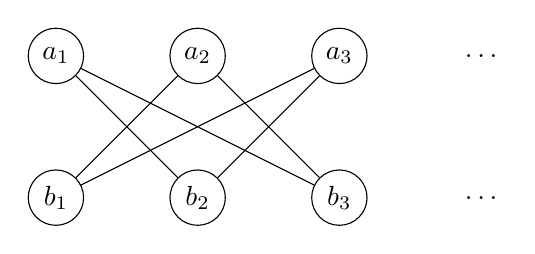
\begin{tikzpicture}[scale=1.2]
        \foreach \i in {1,2,3} {
            \node[circle, draw, minimum size=20pt, inner sep=1pt] (a\i) at (\i*1.5, 1.5) {$a_{\i}$};
            % \node[above=0.1cm of a\i, blue, font=\bfseries] {\i}; % Color label
        }
        \node at (6, 1.5) {$\dots$};
    
        \foreach \i in {1,2,3} {
            \node[circle, draw, minimum size=20pt, inner sep=1pt] (b\i) at (\i*1.5, 0) {$b_{\i}$};
            % \node[below=0.1cm of b\i, blue, font=\bfseries] {\i}; % Color label
        }
        \node at (6, 0) {$\dots$};

        \draw (a1) -- (b2);
        \draw (a1) -- (b3);
        \draw (a2) -- (b1);
        \draw (a2) -- (b3);
        \draw (a3) -- (b1);
        \draw (a3) -- (b2);
    \end{tikzpicture}
\end{figure}
Pokud zvolíme nejpříjemné uspořádání vrcholů \enquote{na střídačku} 
\[
     a_1, b_1, a_2, b_2, a_3, b_3, \dots, a_n, b_n
\]
dostaneme obarvení:
\vspace{-1em}
\begin{itemize}[noitemsep]
    \item $a_1$ nemá obarvené sousedy $\to$ \ii{barva 1}
    \item $b_1$ není spojen s $a_1$ (jediný obarvený), nemá jiné sousedy $\to$ \ii{barva 1}
    \item $a_2$ spojen s $b_1$ (barva 1) $\to$ \ii{barva 2}
    \item $b_2$ spojen s $a_1$ (barva 1), není spojen s $a_2$ $\to$ \ii{barva 2}
    \item[] $\vdots$
    \item $a_k, b_k$ vidí barvy $1, \dots, k-1$ na předchozích vrcholech $\to$ \ii{barva k}
\end{itemize}
\vspace{-1em}
Spotřebujeme tedy $n$ barev (pro $2n$ vrcholů), ačkoliv graf je bipartitní a $\chi(G)=2$.

To se nám oprávněně může zdát jako mnoho. V praxi se osvědčilo, pokud nám vyjde zbytečně mnoho barev, vrcholy \ii{náhodně přeházet} a spustit algoritmus znovu. Toto stačí provést např. 3$\times$ a obvykle dostaneme velmi rozumný počet barev.

\bb{Příklad}. Mějme graf o 7 vrcholech a zvolme uspořádání $6, 1, 2, 3, 5, 7, 4$.

Postupně barvěme
\begin{figure}[H]
    \centering
    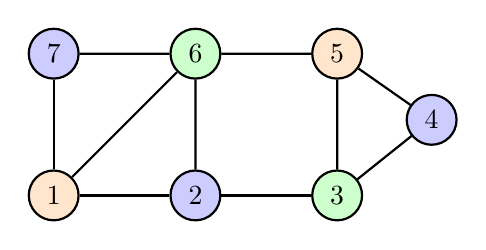
\begin{tikzpicture}[
        scale=1.2,
        vertex/.style={circle, draw, thick, fill=white, minimum size=18pt},
        color1/.style={fill=green!20}, 
        color2/.style={fill=orange!20}, 
        color3/.style={fill=blue!20}    
    ]
        \node[vertex, color2] (1) at (0,0) {1};
        \node[vertex, color3] (2) at (1.5,0) {2};
        \node[vertex, color1] (3) at (3,0) {3};
        \node[vertex, color3] (4) at (4,0.8) {4};
        \node[vertex, color2] (5) at (3,1.5) {5};
        \node[vertex, color1] (6) at (1.5,1.5) {6};
        \node[vertex, color3] (7) at (0,1.5) {7};

        \draw[thick] (7) -- (6);
        \draw[thick] (7) -- (1);
        \draw[thick] (1) -- (6); 
        \draw[thick] (1) -- (2);
        \draw[thick] (6) -- (2);
        \draw[thick] (6) -- (5);
        \draw[thick] (2) -- (3);
        \draw[thick] (5) -- (3);
        \draw[thick] (5) -- (4);
        \draw[thick] (3) -- (4);

        % \node[right] at (5, 1.5) {\textbf{Obarvení:}};
        % \node[right, fill=green!20] at (5, 1.0) {1};
        % \node[right, fill=orange!20] at (5, 0.5) {2};
        % \node[right, fill=blue!20] at (5, 0.0) {3};
    \end{tikzpicture}
\end{figure}
Konkrétní postup barvení:
\begin{center}
    \begin{tabular}{|c|l|c|}
        \hline
        Vrchol & Sousedé (již obarvení) & Barva \\
        \hline
        6 & -- & 1 \\
        1 & 6 (1) & 2 \\
        2 & 1 (2), 6 (1) & 3 \\
        3 & 2 (3) & 1 \\
        5 & 6 (1), 3 (1) & 2 \\
        7 & 6 (1), 1 (2) & 3 \\
        4 & 3 (1), 5 (2) & 3 \\
        \hline
    \end{tabular}
\end{center}
Výsledkem je platné obarvení pomocí 3 barev.

\subsection{Věta o souvislosti největšího stupně vrcholu a barevnosti grafu}\label{brooks}
\ii{Brooks}. Nechť $G$ je prostý \hyperref[souvisly]{souvislý} graf bez smyček, který není ani úplný ani \hyperref[kruznice]{kružnice} liché délky. Pak
\begin{equation}
    \chi(G) \leq \Delta(G).
\end{equation}
\dukaz
Omezme se na $\Delta(G) \geq 3$. Indukcí podle $|V| = n$.
\begin{enumerate}[(a)]
    \item \ii{Základní krok}, $n=4$.
        \begin{figure}[H]
            \centering
            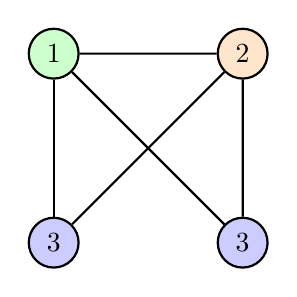
\begin{tikzpicture}[
                scale=1.2,
                vertex/.style={circle, draw, thick, fill=white, minimum size=18pt},
                color1/.style={fill=green!20}, 
                color2/.style={fill=orange!20}, 
                color3/.style={fill=blue!20}    
            ]
                \node[vertex, color1] (1) at (0, 2) {1};
                \node[vertex, color2] (2) at (2, 2) {2};
                \node[vertex, color3] (3) at (0, 0) {3};
                \node[vertex, color3] (4) at (2, 0) {3};

                \draw[thick] (1) -- (2);
                \draw[thick] (2) -- (4);
                \draw[thick] (3) -- (1);

                \draw[thick] (1) -- (4);
                \draw[thick] (2) -- (3);
            \end{tikzpicture}
        \end{figure}
    \item \ii{Indukční předpoklad}. Předpokládejme, že každý souvislý $G^\prime \in \S$, $|V^\prime| = n$, který není $K_n$ a má $\Delta(G^\prime) \geq 3$ se dá obarvit $\Delta(G^\prime)$ barvami.
    \item \ii{Indukční krok}. $G = (V, E)$, $|V| = n + 1$. Zvolme $u_0 \in V$, pak $G \setminus u_0 = H$ je graf o $n$ vrcholech.
    % TODO: dodělat důkaz
\end{enumerate}
